\documentclass{llncs}
\usepackage{makeidx}
\usepackage{cite}
\usepackage{graphicx}
\usepackage{amsmath,amssymb}
\usepackage{subfigure}
%

\begin{document}
\pagestyle{plain}

\mainmatter

\title{Accounting for Heterogeneity Across Multiple Imaging Sites Using Multi-Task Learning}
%
\titlerunning{short title}  % abbreviated title (for running head)
%
% use \inst{1} to get numbered tags on authors to match affiliations
\author{No Author Given}
%\author{Michelle T. Hromatka\inst{1} \and Wei Liu\inst{1}  \and Jeffrey S. Anderson\inst{2} \and Brandon A. Zielinski\inst{3} \and Molly B. DuBray\inst{4} \and P. Thomas Fletcher\inst{1}}
\institute{No Institute given}
%\institute{School of Computing\and Division of Neuroradiology \and Division of Child Neurology\and
%Interdepartmental Program in Neuroscience
%\\ University of Utah, Salt Lake City, UT 84112, USA}

\maketitle

\begin{abstract}
Combining imaging data from multiple sites has the potential to increase statistical power in clinical studies. However, while pooling multiple data sources increases sample size, it also increases unwanted variance due to inconsistencies across sites, e.g., different scanners, protocols, and demographics. In this paper, we present an approach for combining multi-site imaging data in classification tasks that takes this heterogeneity into account. The idea is to treat the classification problem as a multi-task learning problem, where each imaging site is treated as a ``task''. We employ a regularized support vector machine (SVM) that allows for differences in decision boundaries at individual sites, while at the same time leveraging the similarities in the decision boundaries across sites. We demonstrate the effectiveness of this approach in the classification of autism from multi-site functional magnetic resonance imaging (fMRI) from the Autism Brain Imaging Data Exchange (ABIDE). The proposed method achieves state-of-the-art accuracy and outperforms a comparable SVM classifier applied to pooled data as well as individual SVM classifiers applied per site.

% This paper combines traditional learning methods with regularized multi-task learning  to account for the differences between site data while still assuming similarity between tasks.  The ABIDE dataset is used for this research where a third of the data are removed and used to select a variety of parameters which are then used within a leave-one-out SVM classifier for the remaining test subjects. \keywords{SVM classification, ABIDE, Autism, ASD, multi-task learning, multi-site data }
\end{abstract}

\section{Introduction}
Recent years have seen a movement towards combining neuroimaging data collected
across multiple sites. Such multi-site data has the potential to accelerate
scientific discovery by increasing sample sizes, providing broader ranges of
participant demographics, and making data publicly available. Different
approaches include large, coordinated multi-site neuroimaging studies, such as
the Alzheimer's Disease Neuroimaging Initiative (ADNI) \cite{adni}, as well as
data sharing initiatives that combine multiple single-site studies, such as the
Autism Brain Imaging Data Exchange (ABIDE) \cite{abide}. Analysis using these
data sets, however, is not straightforward, due to differences across site
scanners, protocols, populations, and diagnosis techniques. Treating a
multi-site study as a single, homogeneous data set fails to account for this
variability, which can be detrimental to the statistical power and counteract
the gains made by increasing the sample size.

An alternative approach is to perform separate statistical analyses at
individual sites and combine the results in a meta-analysis. This is often
formulated as a random effects model~\cite{DerSimonian}, where each site is
regarded as a random treatment effect. While this can be an effective way to
combine statistical tests of low-dimensional summary measures, it is less
applicable to learning problems on high-dimensional data such as images. For
instance, applying independent classifiers at each site and then combining them
post-hoc misses the opportunity that the classifiers could benefit from sharing
information across sites during learning.  Meta-analysis is also prone to publication bias, meaning only results from
studies whose results were significant enough to publish are aggregated.  By using shared raw data instead of widely
published results, this bias can ideally be avoided \cite{meta}.

In this paper, we propose an approach for combining multiple imaging studies in
classification problems. The idea is to treat the problem as a multi-task
learning problem, where classifiers for each site are estimated jointly, with a
regularization that favors similarity across sites. This allows classifiers to
share information during learning, but also provides the flexibility for them to
differ at each site as needed. This is the key principle in multi-task learning:
heterogeneity across similar tasks (or, in our case, sites) can be accounted for
while using a common mean to account for similarities between the different
tasks. We specifically employ a regularized support vector machine (SVM)
introduced by Evgeniou and Pontil~\cite{regMTL}. As a driving problem, we
apply this method to the classification of autism from functional magnetic
resonance imaging (fMRI) from the ABIDE database.

Several groups have reported classification results using the ABIDE data, in
each case treating the pooled collection of images across all sites as a single
homogeneous data set during classification. Nielsen, et al.~\cite{Jared} combined
the ABIDE data set with a whole-brain approach, using a leave-one-out classifier
to compute a classification score for each left-out subject based on age, gender
and handedness. The correlations for each connection in turn were fit with a
linear model, separating controls from subjects with an Autism Spectrum Disorder (ASD), which was then adjusted by the
difference between the subject's site mean for that connection and the overall
mean. This approach yielded a maximum overall accuracy of 60.0\% despite finding
significant positive correlation between the classification score and several of
the phenotypic behavioral measures \cite{Jared}. A different study used
histogram of gradients and applied this to several multi-site imaging studies
which was able to achieve 61.7\% accuracy on the ABIDE data set and 62.6\% on the
ADHD-200 data set \cite{ghiassian}. While \cite{Jared} accounted for the site
differences during feature generation and selection, both studies approached the
differences across imaging sites as noise instead of extra data that can be
leveraged when classifying an aggregate data set.

% Many researchers fail to take these differences as a****8, but rather as increased noise when treating with the drawback of increased noise due to scanner, protocol and population differences.}

%Previous efforts to combine single-site studies have relied primarily on meta-analysis, in which results across small sites are statistically combined to extract patterns common across the combined sample size. Meta-analysis, however, is not free of subjectivity of data variability, thus this method of combined analysis is also faulty \cite{meta}.

\section{Methods}
We formulate classification of multi-site imaging data as a multi-task learning
problem, where each site, $s = 1, \ldots, S$, is treated as a separate
task. This results in a different classifier for each site, which allows for
variability of decision boundaries across sites. At the same time, a regularization
term in the objective function favors similarities between sites, resulting in
sharing of data across sites during training. We specifically use a regularized
version of SVM, introduced by Evgeniou and Pontil~\cite{regMTL}, which we
describe next. Following that, we describe a process for feature selection in
the case of resting state fMRI, which is an important step to reduce the high
dimensionality of the data.

% SVM parameters through cross-validation and the features to be used in classification (see \ref{subsec:FS}).  These parameters are then used in a leave-one-out classifier on the testing data to determine the algorithm's accuracy, sensitivity and specificity. It is important to note that all parameter tuning and feature selection is done exclusively on the \textit{training} set, and the testing set is only used in the final classification to avoid inflation of results.

\subsection{Multi-Task Learning}
\label{subsec:MTL}
Evgeniou and Pontil~\cite{regMTL} introduce a method of multi-task learning
based on kernel methods typically used for single task learning.  This method
relies on minimizing regularization functions, such as that for SVM, to capture
both overall similarity between tasks and individual task differences. Given $N$
feature vectors $x_i \in \mathbb{R}^d$ with labels $y_i \in \{-1, 1\}$, the
traditional minimization for a soft margin SVM~\cite{svm} is
\begin{equation}
\label{eq:svm}
\arg \min_{w} \frac{1}{2}\|w\|^2 + C \sum_{i=1}^N \xi_i,
\quad\quad \text{subject to:}\,\,\, y_i (w \cdot x_i - b) \geq 1 - \xi_i,\,\xi_i
\geq 0,
\end{equation}
where the weight vector $w$ defines the hyperplane, $(w \cdot x +b)$,
which is the boundary between groups, $C \in \mathbb{R}$ is a constant, and $\xi_i
\in \mathbb{R}$ are slack variables.

For multi-task learning, the relationship between $S$ tasks (or sites, in our
case) must be described, which can be framed as a hierarchical model. This
assumes that each task function comes from a class of probability distributions.
The relationship is defined as
\begin{equation}
\label{eq:sim}
 w_s = w_0 + v_s ,
\end{equation}
where $w_0$ is the mean of the data, and each task $s$ has its own weight
vector, $v_s$. Multi-task learning allows for simultaneous learning of the mean
of all tasks, $w_0$, and each task weight vector, $v_s$, so the minimization
function then becomes
\begin{equation}
\label{eq:mtlsvm}
 C \sum_{s=1}^S \sum_{i=1}^m \xi_{is} + \frac{\lambda_1}{S} \sum_{s=1}^S ||v_s||^2 + \lambda_2||w_0||^2 ,
\end{equation}
where $\lambda_1, \lambda_2$ are positive regularization parameters, and $C$ is
still a constant. For high similarity between tasks, the $v_s$ will be small in
relation to $w_0$; this relationship is described by the hyperparameters
$\lambda_1, \lambda_2$ that must be chosen by the user.

The dual of \eqref{eq:mtlsvm} can be described using a feature mapping
$\phi((x,s)),$ which allows us to relate the dual of a multi-task learning
problem to the dual of \eqref{eq:svm} as
\begin{equation}
\label{eq:mtldual}
\max_{\alpha_{is}}  \left\{ \sum_{i=1}^m\sum_{s=1}^S \alpha_{is} -  \sum_{i=1}^m\sum_{s=1}^S\sum_{j=1}^m\sum_{t=1}^S  \alpha_{is}y_{is}\alpha_{jt}y_{jt}\phi((x,t))      \right\},
\end{equation}
where
\begin{equation}
\phi((x,s)) = \Big(\frac{x}{\sqrt{\mu}}, \underbrace{0,...,0}_{s-1}, x,
\underbrace{0,...,0}_{S-s} \Big), \quad \text{for  } \mu = \frac{S \lambda_2}{\lambda_1} .
\end{equation}
As can be seen in \eqref{eq:mtldual}, this is the same dual problem as for a
single-task SVM, with the data transformed by $\phi((x,s))$ into the multi-task
feature space. This can be implemented as a kernel method, without explicitly
computing the higher-dimensional feature vectors $\phi((x,s))$, since only inner
products between features are needed in the SVM optimization.




\subsection{Feature Selection}
\label{subsec:FS}
Data extraction in imaging studies typically involves very high-dimensional data
spaces.  For fMRI, a typical choice for data is the pairwise correlation between
$n$ predefined regions of the brain.  This yields a dataspace of
$\frac{n(n-1)}{2}$ dimensionality, which, even for a relatively small number of
regions, can be computationally expensive.  Feature selection can reduce
redundancy and increase relevancy of the data while reducing computation time
\cite{featsel}. Rather than select features in the
$\frac{n(n-1)}{2}$-dimensional feature space of correlations, we instead select
from the original $n$ brain regions.


One approach to feature selection in SVM is to use the values of the weight
vector $w$ to choose the most relevant features.  Recall that the decision
boundary in an SVM is defined by $w \cdot x - b$, meaning that the highest
magnitudes in the weight vector denote the features that best define the
decision boundary between groups. This is the basis for the SVM recursive
feature elimination (SVM-RFE) method demonstrated in
\cite{guyon2002gene,abide,ecker2010}: an iterative process where a
user-specified number of features corresponding to the lowest $w$ values are
removed from the feature set after each iteration. We modify SVM-RFE to better
suit the fMRI pairwise correlation data by ranking the features not by the
associated $w$ value of each pairwise correlation, but by the $l^2$-norm of an
entire region's pairwise correlation $w$ vector values. This means for each
region, $r$, we extract the $w$ values for all pairwise correlation datapoints
involving region $r$ and find the $l^2$-norm of these $w$ values. This is done
for all regions in the data set which are then ranked and a user-specifed number
of regions corresponding to the lowest associated $l^2$-norms are removed from
the data set after each iteration.  This approach effectively reduces the data
dimension for feature selection purposes while still leveraging the correlation
data.
%The iteration with the highest overall accuracy on the training set is used to determine which regions should be removed from both the training and testing sets in the classifier.

%A ****** approach is to use a simple hypothesis test to determine which features would be most useful in classification.  Nuisance factors, such as age or ******, should be accounted for prior to the hypothesis test to ideally isolate differences attributed to the disease or disorder being studied.  A linear model is then fit to the training set one feature at a time based on group.  If the coefficient for the group  has a $p < .001$, the feature is kept and used in the SVM classification. This test is done on each feature in turn, ultimately reducing the data into a set that has significant differences between groups.
\section{Evaluation}
\subsection{Data}
The Autism Brain Imaging Data Exchange (ABIDE) database is an online consortium
of resting-state fMRI data from 17 international sites, resulting in
brain imaging data for 539 individuals with ASD and 573 typically developing
(TD) controls \cite{abide}. All ASD subjects were diagnosed by either the Autism
Diagnosis Observation Schedule-General (ADOS-G) or the Autism Diagnostic
Interview-Revised tests and removed from the study if other co-morbid disorders
were present  \cite{abide,lordADOS,lordADIR}.  Further inclusion
details can be found in \cite{abide}.
\subsubsection{Preprocessing}
All data was preprocessed using the Functional Connectomes-1000 preprocessing scripts which includes skull stripping, motion correcting, registration, segmentation and spatial smoothing \cite{fcon}.
%\begin{enumerate}
%\item MRI Deoblique, reorient, skull strip
%\item f-MRI Reorient, motion correct, skull strip, smooth
%\item registration
%\item Segmentation - csf, white matter
%\item extracting global signal, from csf and wm
%\item extract time series, Z-transform correlations
%\item spatial smoothing, register to atlas
%\item some sort of regression
%\end{enumerate}
Twelve subjects were removed because of failure during the preprocessing.  Two OHSU subjects were missing the resting fMRI file and 10 UCLA subjects were missing the anatomical scan file which is required in the preprocessing pipeline. This resulted in 1100 subjects for analysis, 530 ASD and 570 TD controls.
\subsubsection{Data Extraction}
From each subject's postprocessed image, the time series for each of 264 regions is extracted based on Power's regions of interest \cite{Powers}. These 264 regions are spread out among the cerebral cortex, subcortical structures and cerebellum, where each region is a sphere of 5mm in radius and regions are separated by a minimum distance of 10mm so as to avoid detection of a shared signal. The Fisher transformed Pearson correlation coefficient is then found between each region and all other 263 regions, resulting in a 34,716 dimensional feature space for each subject. After feature selection, this number was reduced to 74 regions of the original 264, yielding a final feature space of 2701 features.
\subsection{Results}
We split the ABIDE data into two sets; one half of the data is used for training and the other half is used exclusively to test our approach.  This split is performed at the site level, randomly removing half of the ASD subjects and half of the TD subjects per site, and then aggregating these subjects into a testing set to preserve the ratios between sites and groups across the two data sets.

We present results for three cases: one where each site is classified individually, a second where all site data is pooled and considered a single site and the third using the multi-task learning approach described in Section \ref{subsec:MTL}. For all of the results presented within, a linear kernel is used in the SVM, with the error term parameter, $C$,  determined by cross validation on the training set. Multi-task learning requires an additional parameter, $\mu$, which is also determined through cross validation on the training set. Additionally, the training set is used to determine nuisance factor regression on subject age, and feature selection as described in Section \ref{subsec:FS}. It is important to note that all parameter tuning, feature selection, and nuisance factor regression was performed exclusively on the training set. Involving the testing set in any of these procedures can bias the classifier and inflate the results.

% If don't have time for CV with mu
%For multi-task learning, the results are presented with varying values of $\mu$.  Recall that $\mu$ is defined as $\frac{T\lambda_2}{\lambda_1}$, which is used to compute the mean across all tasks, $w_0$, in the formulation of $\phi((x,t))$. For very small values of $\mu$, the $w_0$ term becomes very large in relation to each task's individualized weight vector, $v_t$, so the problem essentially becomes a single-task learning problem.  The converse, where $\mu$ is very large, approaches the scenario where the tasks are completely unrelated \cite{regMTL}.
%This can be seen in figure ******, where a $mu$ value of ***** corresponds to single task learning and a $mu$ value of ****** corresponds to classifying each task individually.  The ******* indicate our results for single-task learning and the combined accuracy for individual task classification.
%The ideal value for $\mu$ appears to be at ********, where the accuracy reaches a peak of ********.

The multi-task learning approach achieved significantly better overall accuracy
than the single task approach, which in turn improved upon the individual site
classifiers. Using multi-task learning, we classified the ABIDE data with an
overall accuracy of 64.9\%, with 67\% sensitivity and 63\% specificity.  Pooling
all data resulted in 62.9\% overall accuracy, 67\% sensitivity and 59\%
specificity. The summed overall accuracy of each individual site was 58.1\% with
sensitivity of 64\% and specificity of 53\%. The site-by-site accuracies for
pooled, individual, and the proposed multi-task classifiers are shown in
Figure~\ref{fig:acc_bar}.
\begin{figure}
	\centering
	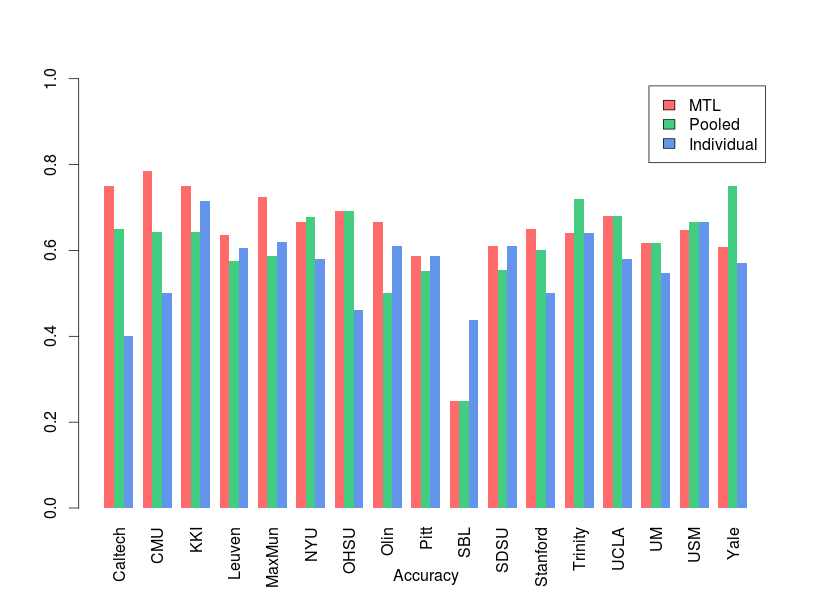
\includegraphics[scale = .4]{acc_bar.png}
	\caption{The overall accuracies by site, as found by each of the three experiments. }
	\label{fig:acc_bar}
	\par\vspace{0pt}
\end{figure}


Several sites benefited greatly from the increase in data size, most notably
Caltech, CMU, MaxMun, and Olin.  All but one of the sites in the bottom 50\% for
sample size either equaled or improved upon the pooled result using multi-task learning.  For
sites that were relatively stable to begin with because of large individual site
sample size (e.g., NYU, UCLA, UM, USM), the multi-task learning approach found little to no
improvement to that site's overall accuracy. This is an expected byproduct of
multi-task learning, as the larger sites already have sufficient data to train
a competent classifier.

\subsection{Visualization of Discriminating Functional Connections}

\begin{figure}[htb]
\begin{minipage}[b]{.6\linewidth}
\centering
%\subfigure[heretoo]{
%\begin{minipage}[b]{0.49\textwidth}
	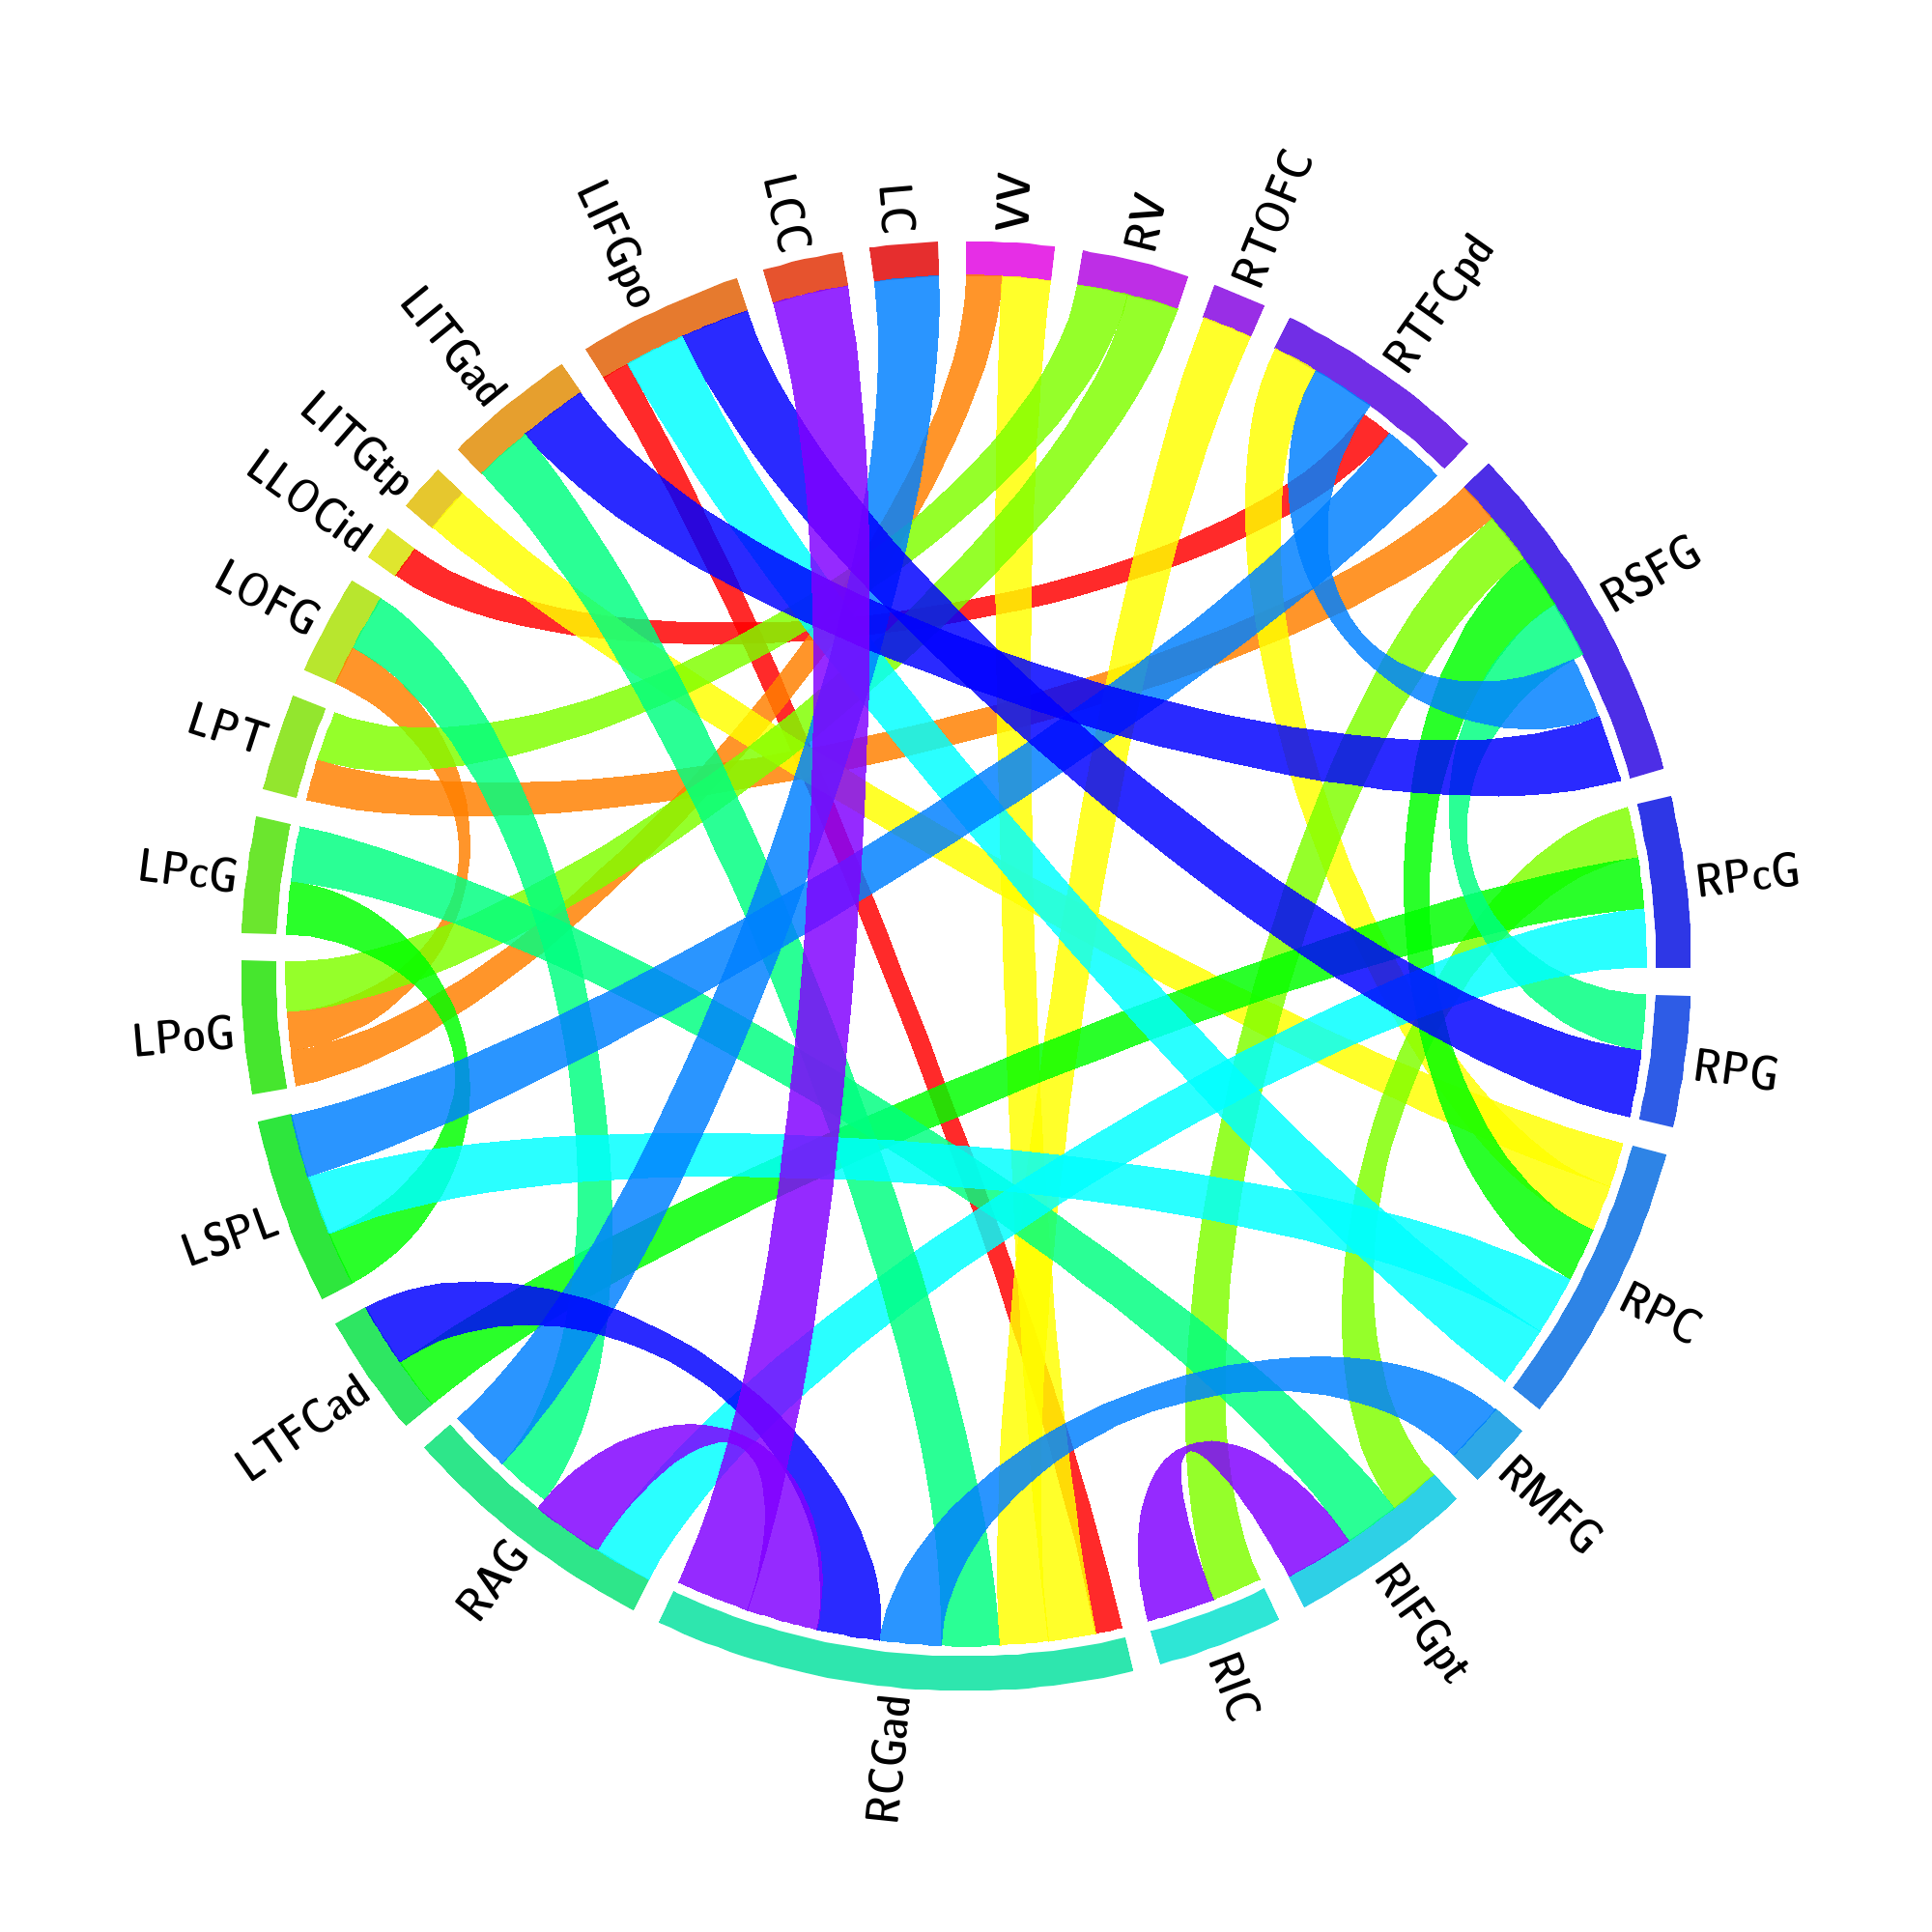
\includegraphics[scale = .11]{now_circos3.png}
	\par\vspace{0pt}
%	}
\end{minipage}
\begin{minipage}[b]{.4\linewidth}
%\begin{table}
%\subtable[stuff]{
\centering
\tiny
\begin{tabular}{l l}
\hline
Abbrev. & Region\\
\hline
LC	& L. Caudate\\
LCC	& L. Cuneal Cortex\\
LCG	& L. Cingulate Gyrus\\
LIC	& L. Insular Cortex\\
LIFG	& L. Inferior Frontal Gyrus\\
LITG	& L. Inferior Temporal Gyrus\\
LLOC	& L. Lateral Occipital Cortex\\
LMTG	& L. Middle Temporal Gyrus\\
LOFG	& L. Occipital Fusiform Gyrus\\
LOP	& L. Occipital Pole\\
LPcG	& L. Paracingulate Gyrus\\
LPG	& L. Precentral Gyrus\\
LPoG	& L. Postcentral Gyrus\\
LPT	& L. Planum Temporale\\
LSFG	& L. Superior Frontal Gyrus\\
LSPL	& L. Superior Parietal Lobule\\
LTFC	& L. Temporal Fusiform Cortex\\
RAG	& R. Angular Gyrus\\
RCG	& R. Cingulate Gyrus\\
RIC	& R. Insular Cortex\\
RIFG	& R. Inferior Frontal Gyrus\\
RITG	& R. Inferior Temporal Gyrus\\
RJLC	& R. Juxtapositional Lobule Cortex\\
RLOC	& R. Lateral Occipital Cortex\\
RMFG	& R. Middle Frontal Gyrus\\
ROP	& R. Occipital Pole\\
RP	& R. Putamen\\
RPC	& R. Precuneous Cortex\\
RPcG	& R. Paracingulate Gyrus\\
RPG	& R. Precentral Gyrus\\
RSFG	& R. Superior Frontal Gyrus\\
RTFC	& R. Temporal Fusiform Cortex\\
RTOFC	& R. Temporal Occipital Fusiform Cortex\\
RV	& R. VI\\
VV	& Vermis VI\\
\hline
ad & anterior division\\
id & inferior division\\
pd & posterior division\\
po & pars opercularis\\
pt & pars triangularis\\
sd & superior division\\
tp & temporooccipital part\\
\hline
\end{tabular}
\par\vspace{0pt}
%}
%\end{table}
\end{minipage}
\caption{The most discriminative pairwise connections as selected by the method described in section \ref{subsec:FS}.  The width of each ribbon is determined by the weights from the $w_0$ vector (i.e., utility) in  specifying the SVM decision boundary. }
%\end{minipage}
\label{fig:circos}
\end{figure}



Figure \ref{fig:circos} displays the regions identified via the method described
in Section \ref{subsec:FS}.  Each ribbon connects two regions whose pairwise
correlation was most discriminative in the SVM classifier, where color and
ribbon width correspond to importance. The regions show a strong overlap with
ROIs previously identified as network ``hubs'' thought to be abnormal in autism,
namely the default mode network (including regions LCGpf, RCGad, RPC) and
socioemotional salience network (including regions RIC, LPcG, RPcG, RIFGpt).
Specifically, these regions include atypical network structure identified in
previous studies of autism using structural covariance MRI
\cite{zielinski2012scmri} and also resting state fMRI (reviewed in
\cite{jeff2014}). It is hypothesized that these abnormal networks may contribute
to many of the behaviors associated with the disorder.

\section{Conclusion}
We presented a novel way to classify multi-site data, specifically neuroimaging
fMRI data, in a way that leverages similarity across sites while accounting for
individual site differences.  Additionally, we introduced a feature selection
approach that is better equipped to handle fMRI pairwise correlation data.  The
utility of these ideas was demonstrated by achieving state-of-the-art
classification accuracy on the ABIDE data set. The results suggest that
multi-task learning can especially benefit imaging sites with smaller sample
sizes.


\bibliography{miccai}{}
\bibliographystyle{plain}





\end{document}
